\documentclass{standalone}
\usepackage{tikz}
\usetikzlibrary{patterns, positioning}
\usepackage[sfdefault]{ClearSans} %% option 'sfdefault' activates Clear Sans as the default text font
\usepackage[T1]{fontenc}

\begin{document}
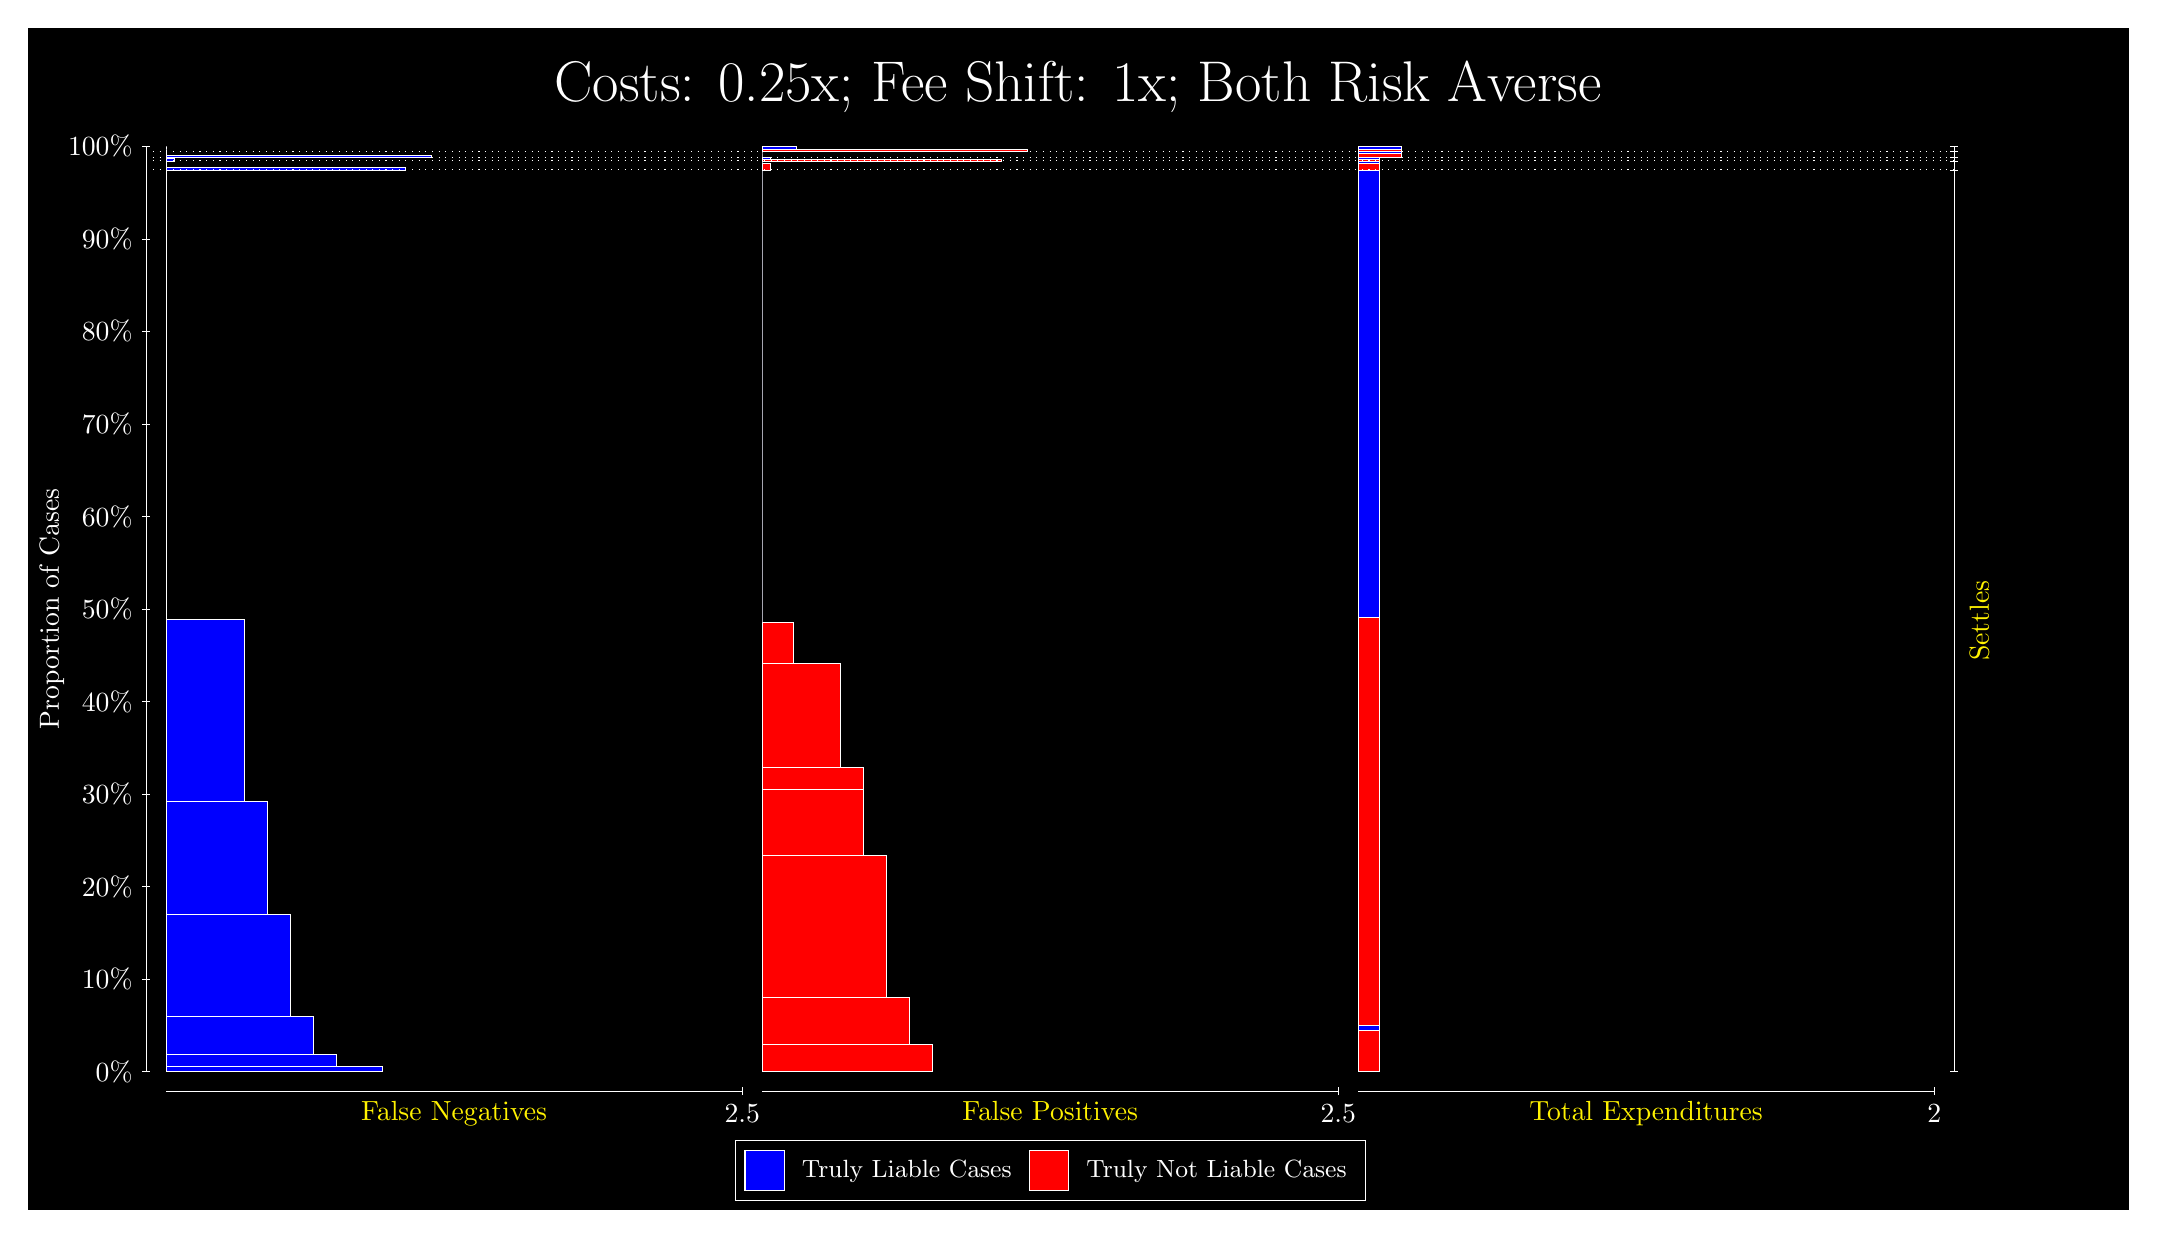
\begin{tikzpicture}
\draw[fill=black] (0,0) rectangle (26.667,15);
\draw[text=white] (0,13.5) rectangle (26.667,15) node[midway] {\huge Costs: 0.25x; Fee Shift: 1x; Both Risk Averse};
\draw[white, very thin] (1.5,1.75) -- (1.5,13.5);
\node[rotate=90, text=white, anchor=center] at (0.3, 7.625) {Proportion of Cases};
\draw[white, very thin] (1.45,1.75) -- (1.55,1.75);
\node[text=white, anchor=east] at (1.45, 1.75) {0\%};
\draw[white, very thin] (1.45,2.925) -- (1.55,2.925);
\node[text=white, anchor=east] at (1.45, 2.925) {10\%};
\draw[white, very thin] (1.45,4.1) -- (1.55,4.1);
\node[text=white, anchor=east] at (1.45, 4.1) {20\%};
\draw[white, very thin] (1.45,5.275) -- (1.55,5.275);
\node[text=white, anchor=east] at (1.45, 5.275) {30\%};
\draw[white, very thin] (1.45,6.45) -- (1.55,6.45);
\node[text=white, anchor=east] at (1.45, 6.45) {40\%};
\draw[white, very thin] (1.45,7.625) -- (1.55,7.625);
\node[text=white, anchor=east] at (1.45, 7.625) {50\%};
\draw[white, very thin] (1.45,8.8) -- (1.55,8.8);
\node[text=white, anchor=east] at (1.45, 8.8) {60\%};
\draw[white, very thin] (1.45,9.975) -- (1.55,9.975);
\node[text=white, anchor=east] at (1.45, 9.975) {70\%};
\draw[white, very thin] (1.45,11.15) -- (1.55,11.15);
\node[text=white, anchor=east] at (1.45, 11.15) {80\%};
\draw[white, very thin] (1.45,12.325) -- (1.55,12.325);
\node[text=white, anchor=east] at (1.45, 12.325) {90\%};
\draw[white, very thin] (1.45,13.5) -- (1.55,13.5);
\node[text=white, anchor=east] at (1.45, 13.5) {100\%};

\draw[white, very thin] (24.457,1.75) -- (24.457,13.5);
\draw[white, very thin] (24.407,1.75) -- (24.507,1.75);
\node[anchor=west] at (24.407, 1.75) {};
\draw[white, very thin] (24.407,13.201) -- (24.507,13.201);
\node[anchor=west] at (24.407, 13.201) {};
\draw[white, very thin] (24.407,13.316) -- (24.507,13.316);
\node[anchor=west] at (24.407, 13.316) {};
\draw[white, very thin] (24.407,13.362) -- (24.507,13.362);
\node[anchor=west] at (24.407, 13.362) {};
\draw[white, very thin] (24.407,13.434) -- (24.507,13.434);
\node[anchor=west] at (24.407, 13.434) {};
\draw[white, very thin] (24.407,13.5) -- (24.507,13.5);
\node[anchor=west] at (24.407, 13.5) {};

\draw[white, very thin, fill=blue] (1.75,1.75) rectangle (4.4946,1.8121);
\draw[white, very thin, fill=blue] (1.75,1.8121) rectangle (3.9091,1.972);
\draw[white, very thin, fill=blue] (1.75,1.972) rectangle (3.6163,2.4458);
\draw[white, very thin, fill=blue] (1.75,2.4458) rectangle (3.3236,3.7524);
\draw[white, very thin, fill=blue] (1.75,3.7524) rectangle (3.0308,5.1864);
\draw[white, very thin, fill=blue] (1.75,5.1864) rectangle (2.738,7.4988);
\draw[white, very thin, fill=red] (1.75,7.4988) rectangle (1.75,13.201);
\draw[white, very thin, fill=blue] (1.75,13.201) rectangle (4.7873,13.231);
\draw[white, very thin, fill=red] (1.75,13.231) rectangle (1.75,13.316);
\draw[white, very thin, fill=blue] (1.75,13.316) rectangle (1.8598,13.345);
\draw[white, very thin, fill=red] (1.75,13.345) rectangle (1.75,13.362);
\draw[white, very thin, fill=blue] (1.75,13.362) rectangle (5.1167,13.386);
\draw[white, very thin, fill=red] (1.75,13.386) rectangle (1.75,13.434);
\draw[white, very thin, fill=red] (1.75,13.434) rectangle (1.75,13.457);
\draw[white, very thin, fill=blue] (1.75,13.457) rectangle (1.75,13.5);
\draw[white, very thin, fill=red] (9.3189,1.75) rectangle (11.478,2.0998);
\draw[white, very thin, fill=red] (9.3189,2.0998) rectangle (11.185,2.6982);
\draw[white, very thin, fill=red] (9.3189,2.6982) rectangle (10.892,4.5002);
\draw[white, very thin, fill=red] (9.3189,4.5002) rectangle (10.6,5.3323);
\draw[white, very thin, fill=red] (9.3189,5.3323) rectangle (10.6,5.6099);
\draw[white, very thin, fill=red] (9.3189,5.6099) rectangle (10.307,6.9299);
\draw[white, very thin, fill=red] (9.3189,6.9299) rectangle (9.7214,7.4524);
\draw[white, very thin, fill=blue] (9.3189,7.4524) rectangle (9.3189,13.201);
\draw[white, very thin, fill=red] (9.3189,13.201) rectangle (9.4287,13.286);
\draw[white, very thin, fill=blue] (9.3189,13.286) rectangle (9.3189,13.316);
\draw[white, very thin, fill=red] (9.3189,13.316) rectangle (12.356,13.333);
\draw[white, very thin, fill=blue] (9.3189,13.333) rectangle (9.4287,13.362);
\draw[white, very thin, fill=red] (9.3189,13.362) rectangle (9.3189,13.41);
\draw[white, very thin, fill=blue] (9.3189,13.41) rectangle (9.3189,13.434);
\draw[white, very thin, fill=red] (9.3189,13.434) rectangle (12.686,13.457);
\draw[white, very thin, fill=blue] (9.3189,13.457) rectangle (9.758,13.5);
\draw[white, very thin, fill=red] (16.888,1.75) rectangle (17.162,2.2725);
\draw[white, very thin, fill=blue] (16.888,2.2725) rectangle (17.162,2.3346);
\draw[white, very thin, fill=red] (16.888,2.3346) rectangle (17.162,7.5145);
\draw[white, very thin, fill=blue] (16.888,7.5145) rectangle (17.162,13.201);
\draw[white, very thin, fill=red] (16.888,13.201) rectangle (17.162,13.286);
\draw[white, very thin, fill=blue] (16.888,13.286) rectangle (17.162,13.316);
\draw[white, very thin, fill=red] (16.888,13.316) rectangle (17.162,13.333);
\draw[white, very thin, fill=blue] (16.888,13.333) rectangle (17.162,13.362);
\draw[white, very thin, fill=red] (16.888,13.362) rectangle (17.437,13.41);
\draw[white, very thin, fill=blue] (16.888,13.41) rectangle (17.437,13.434);
\draw[white, very thin, fill=red] (16.888,13.434) rectangle (17.437,13.457);
\draw[white, very thin, fill=blue] (16.888,13.457) rectangle (17.437,13.5);
\draw[white, dotted] (1.5,13.201) -- (24.457,13.201);
\draw[white, dotted] (1.5,13.316) -- (24.457,13.316);
\draw[white, dotted] (1.5,13.362) -- (24.457,13.362);
\draw[white, dotted] (1.5,13.434) -- (24.457,13.434);
\draw[white, very thin] (1.75,1.5) -- (9.0689,1.5);
\node[text=yellow, anchor=north] at (5.4094, 1.5) {False Negatives};
\draw[white, very thin] (9.0689,1.45) -- (9.0689,1.55);
\node[text=white, anchor=north] at (9.0689, 1.45) {2.5};

\draw[white, very thin] (9.3189,1.5) -- (16.638,1.5);
\node[text=yellow, anchor=north] at (12.978, 1.5) {False Positives};
\draw[white, very thin] (16.638,1.45) -- (16.638,1.55);
\node[text=white, anchor=north] at (16.638, 1.45) {2.5};

\draw[white, very thin] (16.888,1.5) -- (24.207,1.5);
\node[text=yellow, anchor=north] at (20.547, 1.5) {Total Expenditures};
\draw[white, very thin] (24.207,1.45) -- (24.207,1.55);
\node[text=white, anchor=north] at (24.207, 1.45) {2};

\node[text=yellow, centered, rotate=90] at (24.777, 7.4756) {Settles};





\draw (12.978300999999998,1.5) node[draw=none] (baseCoordinate) {};
\begin{scope}[align=center]
        \matrix[scale=0.5, draw=white, below=0.5cm of baseCoordinate, nodes={draw}, column sep=0.1cm]{
            \node[rectangle, draw, minimum width=0.5cm, minimum height=0.5cm, fill=blue] {}; &
            \node[draw=none, font=\small, text=white] (B) {Truly Liable Cases}; &
            \node[rectangle, draw, minimum width=0.5cm, minimum height=0.5cm, fill=red] {}; &
            \node[draw=none, font=\small, text=white] (B) {Truly Not Liable Cases}; \\
            };
\end{scope}

\end{tikzpicture}
\end{document}